\section{Implementation}
The system architecture proposed during the design stages has been divided into three distinct sections for development; services, API and UI. Figure \ref{fig:architecture-changes} shows how the original architecture has been adapted for the development of the prototype.

\begin{figure}[h!]
  \centering
  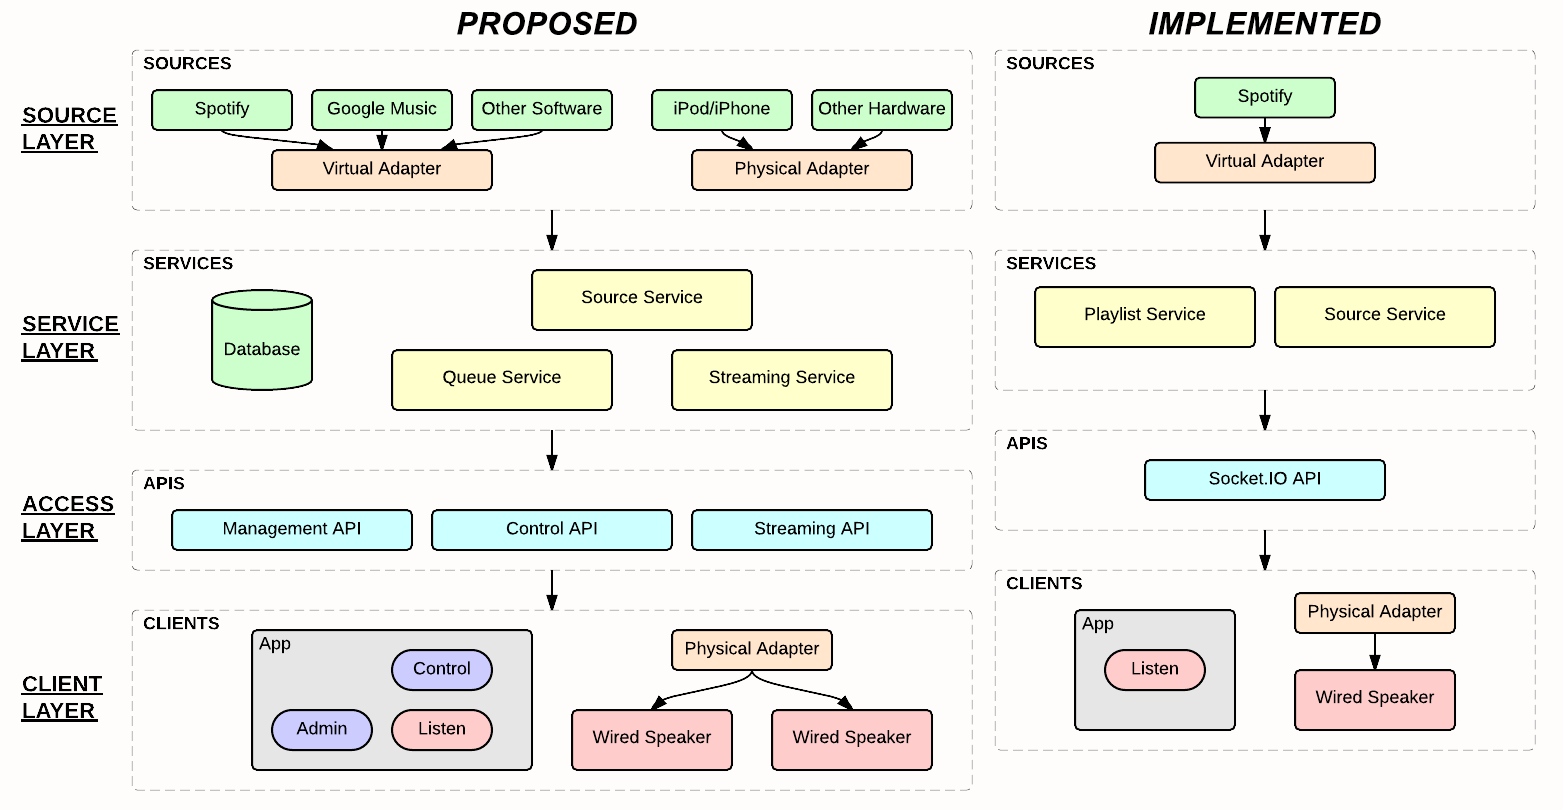
\includegraphics[width=1.02\textwidth]{./img/architecture-changes.png}
  \caption{Prototype architecture alongside original proposed architecture}
  \label{fig:architecture-changes}
\end{figure}

Spotify has been chosen for use as the first type of audio source due to it's well documented and accessible API, along with it's popularity as a personal music service. No physical audio sources, such as iPods, will be available in the prototype due to the added complexity of interfacing with a physical device.

The queue and streaming services have been joined together to create a single playlist service. This is because the contexts of the two services are very similar and can be regarded as tightly-coupled in functionality; the micro-services architecture specifies\footcite{microservicesio} that services should be de-coupled in order to promote scaling and flexibility.

All three types of APIs have been implemented as one singular Socket.IO API for the purposes of the prototype in an effort to make authentication simpler.

Finally, the management and control part of the mobile app has not been implemented due to time constraints; users will only be able to add songs, up-vote/down-vote tracks and listen to audio.

\clearpage
\subsection{Inter-Service Communication}

As discussed during the design stages, the micro services architecture offers many advantages over traditional monolithic software. By having everything in the system running as a service it is possible to scale the application in every direction with relative ease. It does, however, introduce the complex problem of inter-service communication. Early implementations of the architecture made use of HTTP APIs\footcite{microservices-mueller} which work well in simple applications. Relying on HTTP, however, can be seen as a restriction since it is a one-to-one client-to-server connection. In large scale applications it is often necessary to have one-to-many messaging between many different services. HTTP also requires each service to know how to connect to all other services it wants to communicate with, as shown in figure \ref{fig:http-communication}.

\begin{figure}[h!]
  \centering
  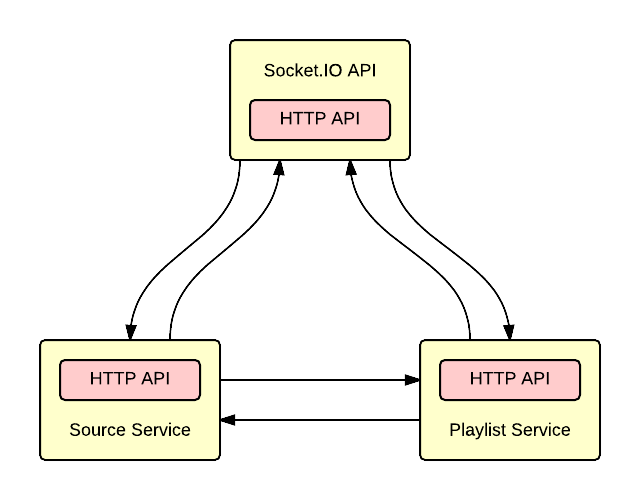
\includegraphics[width=0.6\textwidth]{./img/http.png}
  \caption{Inter-service communication using HTTP APIs}
  \label{fig:http-communication}
\end{figure}

The most popular alternative to HTTP APIs for inter-service communication is a message broker, such as RabbitMQ\footcite{rabbitmq} or Redis\footcite{redis}. In this kind of system, all nodes connect a central broker that is responsible for distributing messages. This has the advantage of a node only needing to know the location of the broker, rather than all other nodes. It also means that messages can be distributed to multiple nodes, removing the one-to-one restriction found in an HTTP-based communication system. Figure \ref{fig:redis-communication} shows how a redis-based communication system can be composed.

\begin{figure}[h!]
  \centering
  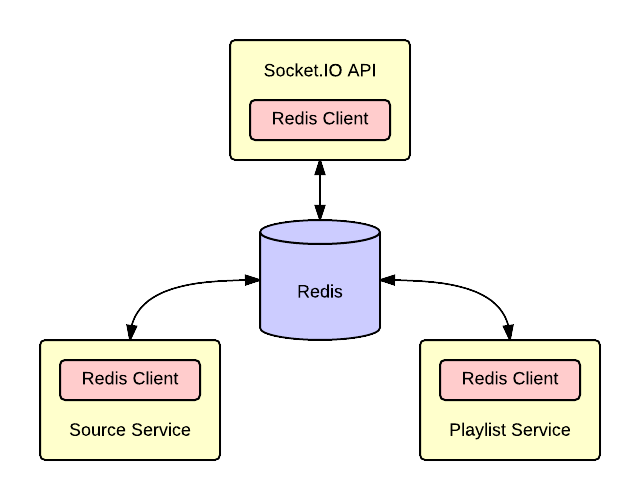
\includegraphics[width=0.6\textwidth]{./img/redis.png}
  \caption{Inter-service communication using Redis}
  \label{fig:redis-communication}
\end{figure}

Messaging systems solve the problem of distributed inter-service communication, however they do introduce their own restrictions. Messages are very low-level; they are simply a single piece of data being transferred between two points. They are entirely stateless and do not support any kind of meta data. It is therefore necessary to treat a service like Redis as a transport and implement a higher-level protocol on top.

This has been achieved in Choona by creating a new communication library called Waterway\footcite{waterway}, built on top of Redis. The roles for both Waterway and Redis can be defined as follows:

\textbf{Waterway:}
\begin{itemize}
  \item Expose an API for three types of high-level messages:
    \begin{itemize}
      \item Streams: a continuous flow of individual messages (such as audio data)
      \item Requests: a single message with a guaranteed response (synonymous to an HTTP request)
      \item Events: a single message with no response (such as a status report)
    \end{itemize}
  \item Translate between high-level messages and low-level redis messages, identified with keys
\end{itemize}

\textbf{Redis:}
\begin{itemize}
  \item Provide an open transport for any type of data to be sent as a message
  \item Distribute messages to nodes by pattern matching the message keys
\end{itemize}

As shown by figure \ref{fig:waterway-communication}, Waterway replaces the role of the standard Redis client in a service. This is where the translation between high-level Waterway messages and low-level Redis messages occurs.

\begin{figure}[h!]
  \centering
  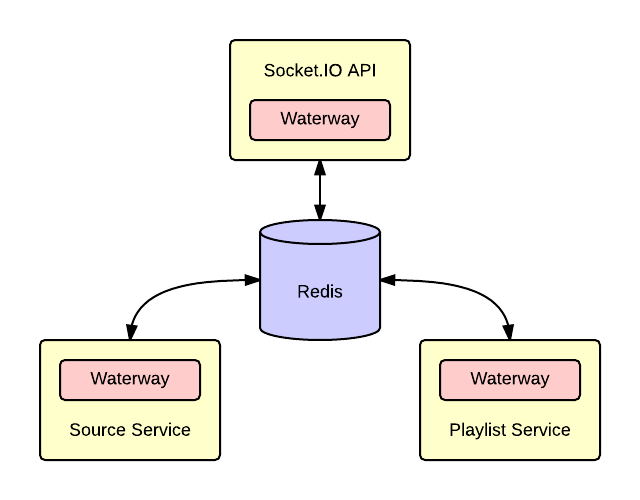
\includegraphics[width=0.6\textwidth]{./img/waterway.png}
  \caption{Inter-service communication using Waterway}
  \label{fig:waterway-communication}
\end{figure}


\subsection{Audio Streaming}

Choona allows multiple clients to connect and listen to the same audio stream. This means that each client needs to be listening to the same audio at the same time, otherwise the whole system will become out of sync. The easiest way to achieve this is to always ensure the audio is being broadcast live, with a very small buffer window (in the same way that when watching television you always see what everyone else does). Waterway makes this process relatively simple due to it's support of streams. As soon as the audio data is received from an audio source such as Spotify it is buffered and streamed out to other services at the exact bitrate of the song. This ensures that all services in Choona see the exact same audio data and the exact same time. It also has the added advantage of allowing the playlist service to know precisely when a track starts and stops; it can just wait for the buffered audio stream to end. Choona's streaming pipeline is described in figure \ref{fig:streaming}.

\begin{figure}[h!]
  \centering
  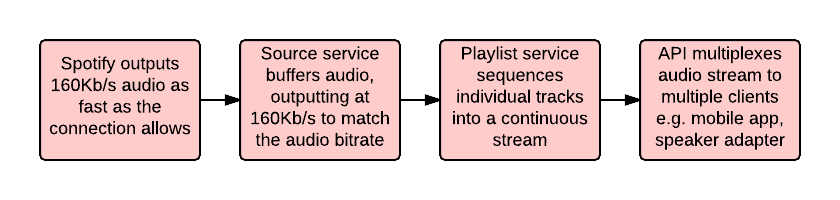
\includegraphics[width=1\textwidth]{./img/streaming.png}
  \caption{Buffered audio streaming through the Choona audio pipeline}
  \label{fig:streaming}
\end{figure}

Clients can then choose to handle the audio in whatever method they prefer; for example, in a browser-based environment the MP3 stream can be converted into raw PCM audio data and played out of the device using the HTML5 Audio API.


\subsection{API}

Socket.IO is a realtime bi-directional communication protocol and library, designed to replace standard HTTP-based web communication. For Choona, Socket.IO offers the following benefits:

\begin{itemize}
  \item \textbf{Bi-directional communication:} HTTP is a client to server model, where only the client can initiate requests. This is fine for regular websites, however it does not work for scenarios where the server needs to send requests without the client initiating them, such as a realtime application like Choona. To counter this there are now several different strategies and protocols for handling bi-directional communication on the web, many of which are supported by Socket.IO such as WebSockets and long polling.
  \item \textbf{Device support:} Socket.IO will select the best available bi-directional protocol supported by both the client and server when setting up connections, resulting in almost all devices being supported.
  \item \textbf{Binary data support:} As specified in the requirements, the Choona app will need to be able to play audio out of the phone speakers/headphones. This means the audio data will need to be streamed into the app. Socket.IO has built-in support for correctly transferring binary data which means the audio can be streamed using the same communication and authentication methods as the rest of the app.
\end{itemize}

Choona's Socket.IO API acts as a simple gateway between clients (such as the mobile app) and the many services that make up the backend infrastructure. It has three main objectives:

\begin{itemize}
  \item authenticate users
  \item ensure requests are authorised
  \item proxy requests to other services in the system
\end{itemize}

The API can almost be interpreted as a firewall; it protects the internal services from being unauthorised access and ensures users are authenticated. It also means that clients do not and cannot know about the internal structure of Choona's architecture which adds an element of security by secrecy.


\subsection{Authentication}

Choona's user authentication is managed by the SaaS platform Auth0. It is now commonplace for applications to allow users to authenticate with many different third parties such as Facebook and Twitter. Developing and maintaining support for even one type of authentication can often prove to be fairly involved, let alone 3 or 4. Auth0 helps developers with this problem by abstracting all the different authentication providers into a single API, giving many advantages\footcite{auth0}:

\begin{itemize}
  \item Only need to implement one authentication system
  \item Quickly build embedded login forms using the Auth0 libraries
  \item Manage all users from a central management interface (Figure \ref{fig:auth0-users})
  \item Easily maintain a single, common view of the user's data
  \item Integrate with existing user databases
\end{itemize}

\begin{figure}[h!]
  \centering
  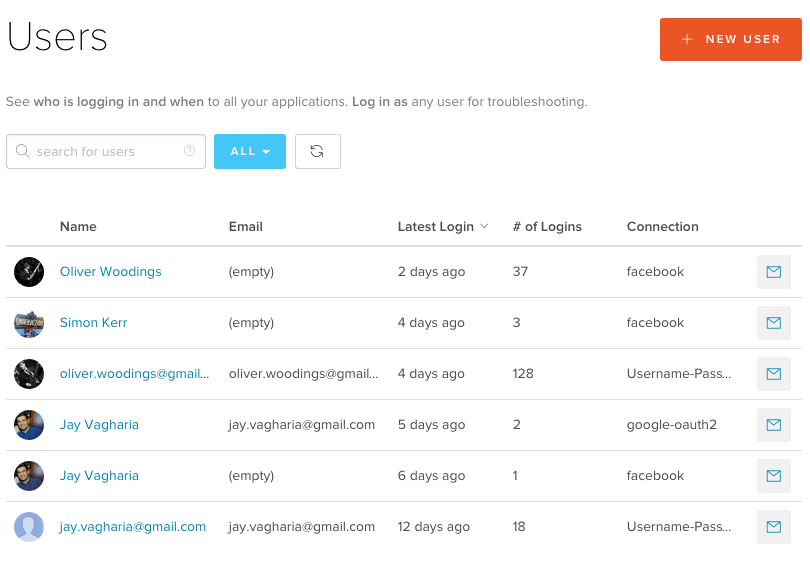
\includegraphics[width=0.6\textwidth]{./img/auth0-users.png}
  \caption{Auth0 user management}
  \label{fig:auth0-users}
\end{figure}

Auth0 handles the entire login and authentication process without needing any changes to an application's server-side systems. This is achieved by using JSON Web Tokens; a unified way of structuring and encoding authentication data into a JSON object. This object is then encrypted using a private key, allowing it's integrity to be easily validated by third parties using the corresponding public key. JSON Web Tokens are used by the Choona API to ensure a user is authenticated and also to extract information about them for use in other services. This process is shown in figure \ref{fig:auth-process}.

\begin{figure}[h!]
  \centering
  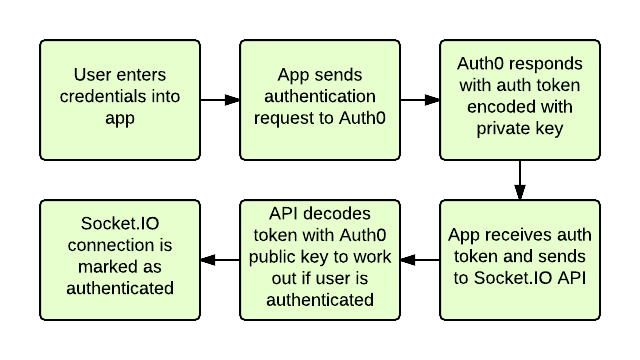
\includegraphics[width=0.7\textwidth]{./img/auth-process.png}
  \caption{Choona authentication process}
  \label{fig:auth-process}
\end{figure}


\subsection{Speaker Adapter}

As part of this first iteration of development a prototype of a Choona speaker adapter has been made. The hardware used is a Raspberry Pi 2 Model B running the Raspbian operating system. The software itself is designed to be as autonomous as possible; once the device has an internet connection it will automatically connect to the Choona API, authenticate and start streaming to music from the pre-configured playlist. This is then outputted from the jack socket of the Raspberry Pi into whatever speakers or headphones are connected.


\subsection{UI}

The Choona mobile app is made using the Ionic framework, which itself is built on top of AngularJS. As discussed in the design stages, building a mobile app using web-based technology allows it to easily be deployed to any platform. Ionic makes this even easier by making available a set of mobile-friendly UI components\footcite{ionic}. Figure \ref{fig:phonegap} shows how PhoneGap/Cordova is used to take the Choona source code and compile it into ready-to-deploy applications for each mobile platform.

The app itself is structured like a typical AngularJS application, using factories, states, controllers, scopes and views:

\begin{itemize}
  \item \textbf{Factory:} a constructor that instantiates or prepares an object for use in the rest of the app
  \item \textbf{State:} a component of the routing state machine used to navigate around the application and render different views\footcite{router}
  \item \textbf{Controller:} responsible for interfacing between views and the rest of the app
  \item \textbf{Scope:} each controller/state has it's own scope for containing variables and methods, which is inherited and extended from parent scopes
  \item \textbf{View:} HTML mixed in with Angular's data binding syntax
\end{itemize}

\begin{figure}[h!]
  \centering
  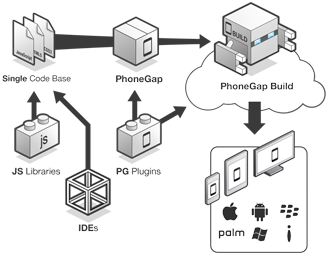
\includegraphics[width=0.5\textwidth]{./img/phonegap.png}
  \caption{PhoneGap/Cordova build process\footcite{phonegap}}
  \label{fig:phonegap}
\end{figure}

Figure \ref{fig:state} shows Choona's application state/scope tree. Children inherit the scopes of their parents, which makes it possible to pass properties and methods from the root scope all the way down to nodes at the bottom of the tree. This inheritance also makes it simple to implement authentication restrictions; by applying the restriction in the App state the application will also inherently prevent access to all the child states.

\begin{figure}[h!]
  \centering
  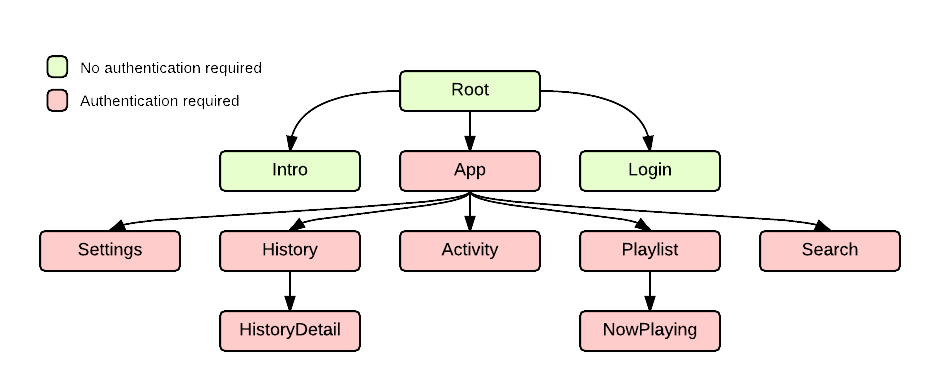
\includegraphics[width=0.9\textwidth]{./img/state.png}
  \caption{Choona's application state/scope tree}
  \label{fig:state}
\end{figure}

Scope inheritance is used in Choona to share data between controllers and views, creating a \textit{single source of truth}. This is achieved by storing application-wide data on the highest possible node in the tree; in this case it is the App state. For example, the current playlist information is stores on the App scope since it is required by both the Playlist and History states. If the data was stored on each node individually it would create two different sources of truth that would both need to be maintained separately. All data received from the Socket.IO API is stored at the application level in order to preserve this single source of truth. When data needs to be sent back to the Socket.IO API it is the responsibility of the closest controller/scope to the source of the action. For example if a user upvotes a song on the playlist, it is the role of the playlist controller to inform the API about the change. This whole process is the \textit{data lifecycle} of Choona, and is visualised in figure \ref{fig:lifecycle}.

\begin{figure}[h!]
  \centering
  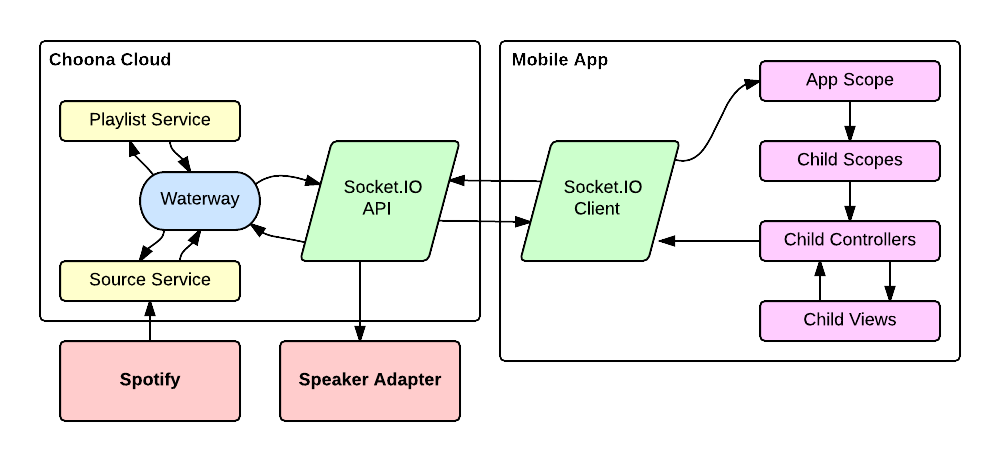
\includegraphics[width=0.9\textwidth]{./img/lifecycle.png}
  \caption{Data lifecycle of the entire Choona ecosystem}
  \label{fig:lifecycle}
\end{figure}